\section{Popis součástí}

Trezor má tvar krychle o~délce hrany 128~mm, násobek šestnácti jsem zvolil kvůli jednoduché návaznosti na dřívka, %todo přidáme pár vět o dřívkách 
dřevěná dřívka s obdélníkovým průřezem 3x16~mm nebo 2x16~mm. 
    %Tyto dřívka používáme s dětmi na Robotárně se skvělým ohlasem, již několik led. 
    %Jdná se vlastně o dřevění odpad ze kterého se ale nádherně staví nejrůznější modely, nebo jednoduše a velmi rychle vyrobitelné dodatky k robotům.
    %% nevím ale moc víc mě ke dřívkům nenapadá 
Protože je trezor vyroben z překližky o~síle 4~mm, jsou jeho vnitřní rozměry o 4~mm na každé straně menší (takže 122~mm).

Trezor se zamyká pomocí rotační západky a~čtyř kódovacích kol, která blokují západku v zamčeném stavu. 
Princip mechanizmu je na obrázku \obr{fig:M2-mechanizmus}.

\paragraph{Geometrie západky}
\begin{figure}[h]
	\centering
    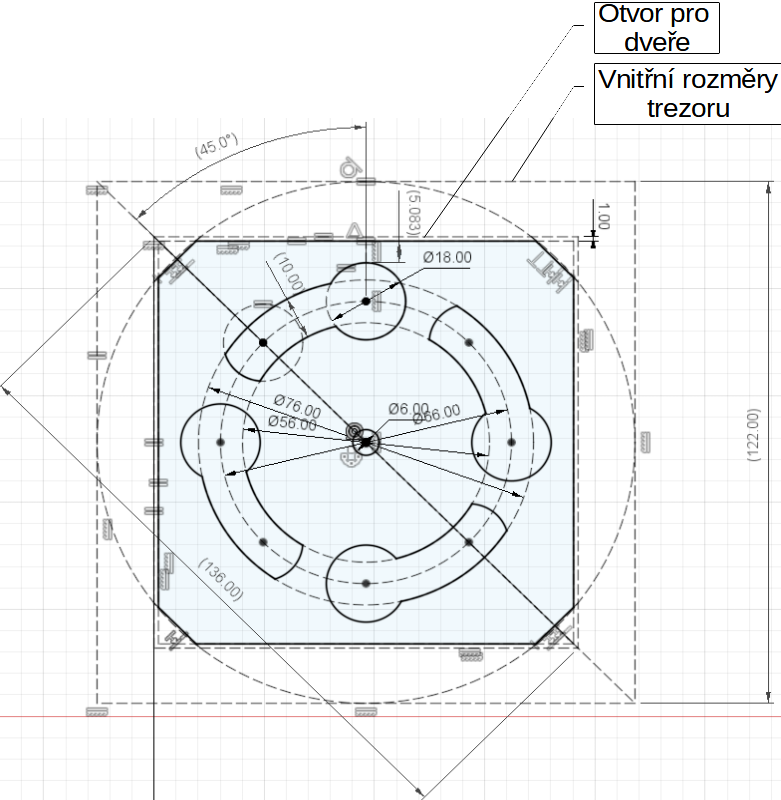
\includegraphics[width=0.7\textwidth]{kapitoly/obrazky/M3/geometrie_zapadky.png}
    \caption{Náčrt západky}
    \label{fig:M3-geometrie-zapadky}
\end{figure} 

Protože se západka otáčí, musí pro ni být zajištěn dostatek prostoru, zároveň však otvor pro dveře je lepší mít větší, protože se potom trezor dá použít pro větší objekty.
Z tohoto důvod jsou hrany západky definovány kružnicí o~průměru délky vnitřní hrany trezoru. Západka má v~rozích sražení ze dvou důvodů. Za prvé, aby byl otvor pro
dveře větší a~za~druhé, aby namáhání působící v~západce působilo na větší délce.

\newpage

\paragraph{Distanční deska}

Aby se západka dostala za desku přední stěny bedny trezoru, je potřeba jí od přední stěny dveří posunout právě o tloušťku stěny. To zajišťuje jednoduchá čtvercová deska jen s~pěti otvory
pro průchod ovládacích kol.

\begin{figure}
	\centering
    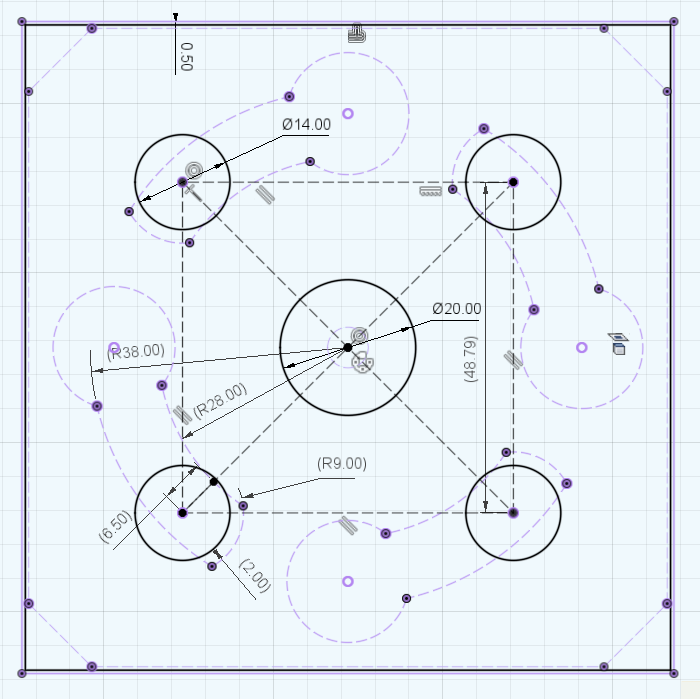
\includegraphics[width=0.7\textwidth]{kapitoly/obrazky/M3/distancka.png}
    \caption{Náčrt distanční desky}
    \label{fig:M3-distancka}
\end{figure}

\paragraph{Stavitka}
\begin{figure}
	\centering
    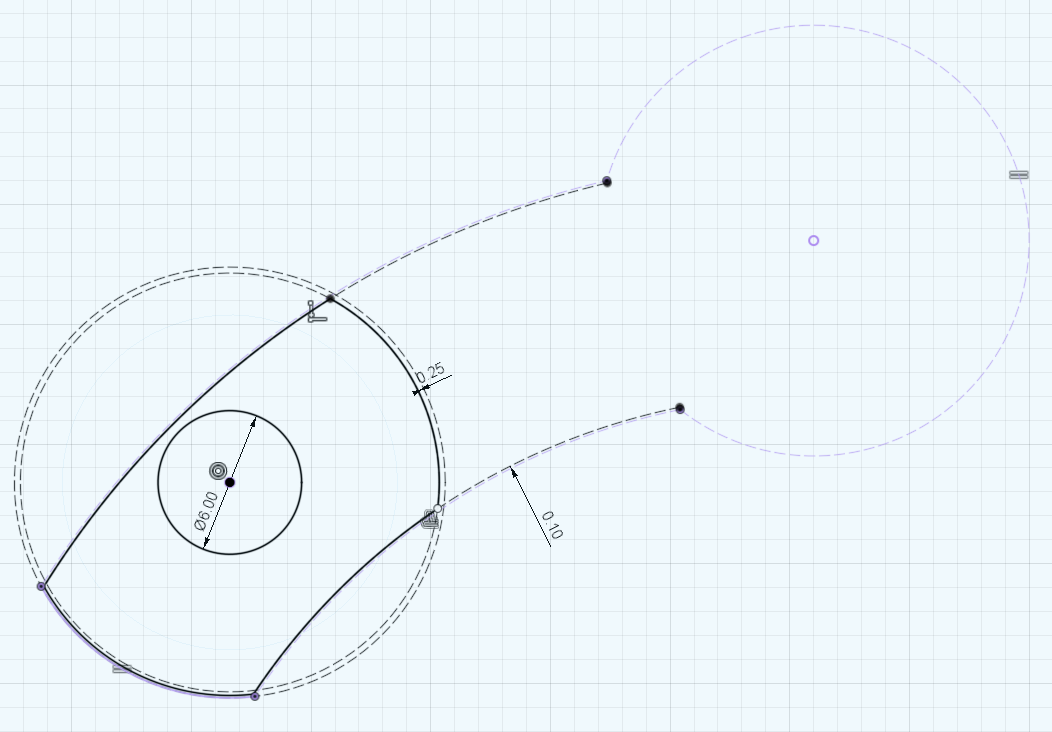
\includegraphics[width=0.7\textwidth]{kapitoly/obrazky/M3/kamen.png}
    \caption{Náčrt stavítka}
    \label{fig:M3-kamen}
\end{figure}

Stavítko, který zajišťuje kód, má z~části tvar drážky, ve které jezdí, a~z~části kruh, který se~muže otáčet v~kruhovém otvoru na jedné staně drážky.
Uprostřed má~kruhový otvor o~průměru 8~mm pro kolík, který stavítkem otáčí.

\paragraph{Lepící distanční kroužek}

\begin{figure}[h]
	\centering
    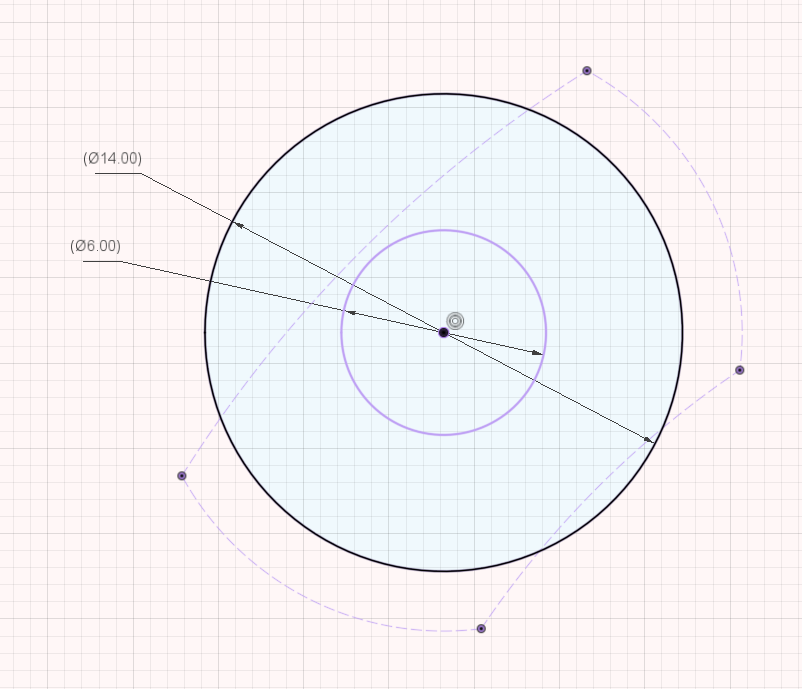
\includegraphics[width=0.7\textwidth]{kapitoly/obrazky/M3/lepici_distance.png}
    \caption{Náčrt lepícího distančního kroužku}
    \label{fig:M3-lepici-distance}
\end{figure}

Tyto distanční kroužky jsou zde čistě z~technologického důvodu. Při lepení kolíku totiž měly děti problém s~lepidlem, které jim zatékalo do~prostoru mezi kolíkem 
a~stěnou dveří, čímž znemožňovalo otáčení kol. Proto jsem přidal tyto kroužky, do~kterých když zateče lepidlo, tak~se nic neděje.

\newpage